% ============================================================
% Recueil COMIMa — Techniques de résolution de problèmes
% Chapitre 6 — Combinatoire
%
% Compilation (paquet .tex exporté) : latexmk -pdf cours.tex
% Les énoncés des exercices sont inclus depuis <id>/enonce.tex
% (content/exercices/ sur le dépôt).
% ============================================================
\documentclass[11pt]{article}
\input{preamble.tex}
\input{preamble-cours.tex}

% Solutions en fin de chapitre : \solutionsfalse pour les masquer.
\solutionstrue

\begin{document}

\chapitre{6}{Combinatoire}

La combinatoire consiste à \emph{compter sans énumérer un à un}.
Les deux premiers outils sont le \textbf{principe additif} et le
\textbf{principe multiplicatif}.

% ------------------------------------------------------------
\section{Exemples introductifs}\label{sec:exemples-introductifs}

\subsection{Les principes additif et multiplicatif}\label{sec:principes-additif-multiplicatif}

\begin{theoreme}[Principe additif]\label{thm:additif}
Lorsqu’un choix se fait \emph{dans une catégorie ou dans une autre}, ces catégories n’ayant
aucun choix en commun, on additionne les nombres de choix.
\end{theoreme}

\begin{exemple}
À la sortie du lycée, Tiana peut acheter un goûter :
\begin{itemize}
    \item un \emph{koba} parmi \(3\) sortes ;
    \item ou un \emph{mokary} parmi \(2\) sortes.
\end{itemize}
Combien de choix a-t-il ?
\end{exemple}

\begin{solution}
\[
3+2=5.
\]

Il y a donc \(\boxed{5}\) choix possibles.
\end{solution}

\begin{theoreme}[Principe multiplicatif]\label{thm:multiplicatif}
Lorsqu’un choix se fait en plusieurs étapes successives, et que le nombre de possibilités
à chaque étape ne dépend pas des choix déjà faits, on multiplie.
\end{theoreme}

\begin{exemple}
Sur son chemin, Tiana peut composer son repas avec :
\begin{itemize}
    \item un plat parmi \(3\) possibilités : \emph{romazava}, \emph{ravitoto}, \emph{vary amin’anana} ;
    \item une boisson parmi \(2\) possibilités : eau ou jus.
\end{itemize}
Le nombre de repas possibles est
\[
3\times 2=6.
\]

Il y a donc \(\boxed{6}\) repas différents.
\end{exemple}

\begin{proposition}[Première généralisation]\label{prop:generalisation-mult}
Si une expérience se déroule en \(p\) étapes, et qu’il y a respectivement
\(n_1,n_2,\dots,n_p\) choix à chaque étape, alors le nombre total d’issues est
\[
n_1n_2\cdots n_p.
\]
\end{proposition}

\subsection{Le principe de l’arbre des choix}\label{sec:arbre-des-choix}

L’arbre des choix permet de visualiser un raisonnement multiplicatif.

\begin{exemple}[Menu malgache]
On choisit :
\begin{itemize}
    \item une entrée : \emph{sambos} ou \emph{achards} ;
    \item un plat : \emph{romazava} ou \emph{ravitoto} ;
    \item un dessert : \emph{koba} ou \emph{mokary}.
\end{itemize}

Chaque menu correspond à un chemin dans l’arbre ci-dessous.

\begin{center}
\fitfig{%
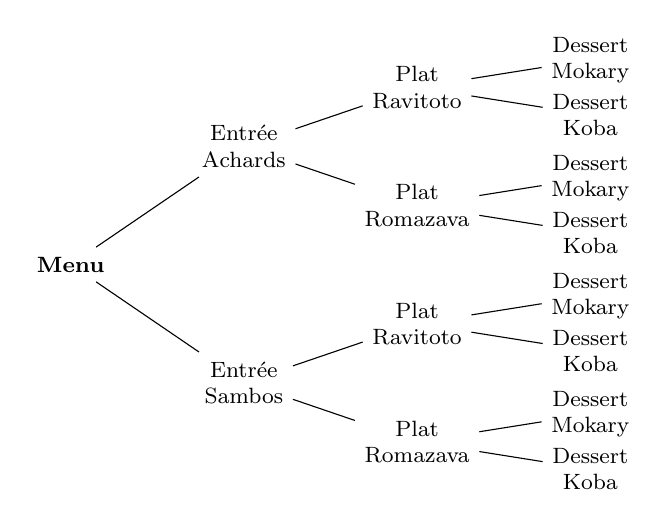
\begin{tikzpicture}[
  grow=right, align=center, font=\footnotesize,
  level 1/.style={sibling distance=30mm,level distance=22mm},
  level 2/.style={sibling distance=15mm,level distance=22mm},
  level 3/.style={sibling distance=7mm,level distance=22mm},
  edge from parent/.style={draw,-}]
\node {\textbf{Menu}}
  child { node {Entrée\\Sambos}
    child { node {Plat\\Romazava} child { node {Dessert\\Koba}} child { node {Dessert\\Mokary}} }
    child { node {Plat\\Ravitoto} child { node {Dessert\\Koba}} child { node {Dessert\\Mokary}} } }
  child { node {Entrée\\Achards}
    child { node {Plat\\Romazava} child { node {Dessert\\Koba}} child { node {Dessert\\Mokary}} }
    child { node {Plat\\Ravitoto} child { node {Dessert\\Koba}} child { node {Dessert\\Mokary}} } };
\end{tikzpicture}}
\end{center}
\end{exemple}

\begin{solution}
Comme il y a \(2\) choix pour l’entrée, \(2\) choix pour le plat et \(2\) choix pour le dessert,
on obtient

\[
2\times 2\times 2=8.
\]

Il y a donc \(\boxed{8}\) menus possibles.
\end{solution}

\begin{remarque}
L’arbre sert surtout à \emph{voir} les possibilités ; le calcul se fait ensuite par multiplication.
\end{remarque}

\subsection{Le principe des codes : avec répétitions et sans répétitions}\label{sec:principe-des-codes}

\paragraph{Codes avec répétition autorisée.}
\begin{exemple}
On forme un code à \(3\) chiffres avec les symboles
\[
0,\;1,\;2,\;3.
\]
Chaque position peut contenir n’importe lequel des \(4\) symboles.

Le nombre de codes est donc
\[
4\times 4\times 4=4^3=64.
\]

Il y a \(\boxed{64}\) codes possibles.
\end{exemple}

\begin{proposition}[Généralisation]\label{prop:codes-avec-repetition}
Si un code est de longueur \(p\) et si l’on dispose de \(n\) symboles, alors avec répétition autorisée,
le nombre total de codes est
\[
\boxed{n^p}.
\]
\end{proposition}

\paragraph{Codes sans répétition.}
\begin{exemple}
On reprend les symboles \(0,1,2,3\), mais cette fois un symbole ne peut pas être utilisé deux fois.

\begin{itemize}
    \item \(4\) choix pour le premier chiffre ;
    \item \(3\) choix pour le deuxième ;
    \item \(2\) choix pour le troisième.
\end{itemize}

Donc
\[
4\times 3\times 2=24.
\]

Il y a \(\boxed{24}\) codes possibles.
\end{exemple}

\begin{proposition}[Généralisation]\label{prop:codes-sans-repetition}
Avec \(n\) symboles distincts et un code de longueur \(p\) sans répétition (avec \(p\le n\)), on obtient
\[
\boxed{n(n-1)(n-2)\cdots(n-p+1)}.
\]
\end{proposition}

Cette quantité apparaîtra plus tard sous le nom d’\emph{arrangement}.

\subsection{Choisir sans ordre et avec ordre}\label{sec:sans-ordre-avec-ordre}

On termine par une distinction fondamentale :
\emph{l’ordre compte-t-il ou non ?}

\subsubsection*{Choix sans ordre}

\begin{exemple}
Dans un \emph{fokontany}, \(n\) habitants se portent volontaires pour représenter le quartier.
On veut en choisir \(2\) (avec \(n\ge 2\)), sans attribuer de rôle particulier.
\end{exemple}

\begin{solution}
Ici, choisir \(\{A,B\}\) revient au même que choisir \(\{B,A\}\) :
\textbf{l’ordre ne compte pas}.

Si l’on comptait avec ordre, on aurait :
\[
n(n-1)
\]
possibilités, car :
\begin{itemize}
    \item \(n\) choix pour la première personne ;
    \item \(n-1\) choix pour la deuxième.
\end{itemize}

Mais chaque paire a été comptée \emph{deux fois} :
\[
(A,B)\quad \text{et}\quad (B,A).
\]
Donc le nombre de choix sans ordre est
\[
\frac{n(n-1)}{2}.
\]
\end{solution}

\begin{definition}[Choisir \(2\) parmi \(n\)]
On note ce nombre \(\binom{n}{2}\) (on lit « \(2\) parmi \(n\) ») :
\[
\binom{n}{2}=\frac{n(n-1)}{2}.
\]
\end{definition}

\begin{exemple}[Exemple numérique]
S’il y a \(n=5\) volontaires, alors
\[
\binom{5}{2}=\frac{5\times 4}{2}=10.
\]
\end{exemple}

\subsubsection*{Choix avec ordre}

\begin{exemple}
Parmi \(n\) candidats, on veut choisir
\begin{itemize}
    \item un \emph{sefo fokontany} ;
    \item puis un adjoint, qui est une autre personne.
\end{itemize}
\end{exemple}

\begin{solution}
Cette fois, les rôles sont différents :
choisir \(A\) comme sefo et \(B\) comme adjoint
n’est pas la même chose que choisir \(B\) comme sefo et \(A\) comme adjoint.

Le nombre de choix est donc
\[
n(n-1).
\]
\end{solution}

\begin{exemple}[Exemple numérique]
Pour \(n=5\) candidats :
\[
5\times 4=20.
\]

Il y a donc \(\boxed{20}\) façons de choisir un sefo fokontany et un adjoint parmi \(5\) personnes.
\end{exemple}

\begin{retenir}
\begin{itemize}
    \item \textbf{Principe additif :} si l’on choisit \emph{ceci ou cela}, sans choix commun aux deux, on additionne.
    \item \textbf{Principe multiplicatif :} si l’on choisit \emph{ceci puis cela}, on multiplie.
    \item \textbf{Arbre des choix :} il permet de visualiser une situation de comptage.
    \item \textbf{Code avec répétition :} avec \(n\) symboles et \(p\) positions, on obtient \(n^p\).
    \item \textbf{Code sans répétition :} avec \(p\le n\), on obtient \(n(n-1)\cdots(n-p+1)\).
    \item \textbf{Choix sans ordre :} pour choisir \(2\) personnes parmi \(n\), on obtient
    \[
    \binom{n}{2}=\frac{n(n-1)}{2}.
    \]
    \item \textbf{Choix avec ordre :} pour deux rôles distincts, on obtient
    \[
    n(n-1).
    \]
\end{itemize}
\end{retenir}

% ------------------------------------------------------------
\section{Factorielle et coefficients binomiaux}\label{sec:factorielle-binomiaux}

Dans cette section, on passe des exemples concrets aux premières formules générales
de combinatoire.

\subsection{Des choix successifs à la factorielle}\label{sec:factorielle}

Supposons que \(n\) personnes doivent se placer en file indienne.

\begin{itemize}
    \item Il y a \(n\) choix pour la première place ;
    \item puis \(n-1\) choix pour la deuxième ;
    \item puis \(n-2\) choix pour la troisième ;
    \item etc. ;
    \item enfin \(1\) choix pour la dernière.
\end{itemize}

Le nombre total de files possibles est donc
\[
n(n-1)(n-2)\cdots 2\cdot 1.
\]

\begin{definition}[Factorielle]\label{def:factorielle}
On introduit alors la notation suivante :
\[
\boxed{n! = n(n-1)(n-2)\cdots 2\cdot 1}
\]
On lit \(n!\) : \emph{\(n\) factorielle}.

Par convention, on pose aussi
\[
\boxed{0! = 1.}
\]
\end{definition}

\begin{definition}[Permutation]\label{def:permutation}
Un rangement de \(n\) objets distincts dans un ordre s’appelle une \emph{permutation}
de ces objets.
\end{definition}

\begin{proposition}[Nombre de permutations]\label{prop:permutations}
Il y a \(n!\) permutations de \(n\) objets distincts.
\end{proposition}

\begin{exemple}
Avec \(4\) élèves, le nombre de façons de se ranger est
\[
4! = 4\times 3\times 2\times 1 = 24.
\]
\end{exemple}

\begin{exemple}
Dans un \emph{fokontany}, \(5\) personnes doivent occuper \(5\) rôles distincts
(sefo, adjoint, secrétaire, trésorier, conseiller).
Le nombre d’affectations possibles est
\[
5! = 120.
\]
\end{exemple}

\subsection{Schéma d’ensemble}\label{sec:schema-ensemble}

On peut résumer l’idée générale par le schéma suivant :

\begin{center}
\fbox{
\begin{minipage}{0.94\linewidth}
\[
\resizebox{\linewidth}{!}{$\displaystyle
\boxed{\text{choix successifs}}
\;\Longrightarrow\;
\boxed{n!}
\;\Longrightarrow\;
\boxed{\text{\footnotesize{choix ordonné de} }k\text{\footnotesize{ personnes parmi } }n}
\;\Longrightarrow\;
\boxed{\binom{n}{k}}
$}
\]
\end{minipage}
}
\end{center}

Autrement dit :
\begin{itemize}
    \item quand on choisit \emph{successivement} plusieurs personnes, on multiplie ;
    \item quand on choisit \emph{toutes} les \(n\) personnes dans un ordre, on obtient \(n!\) ;
    \item quand on choisit seulement \(k\) personnes dans un ordre, on obtient un produit plus court (voir ci-après) ;
\end{itemize}

\subsection{Choix ordonné de \(k\) personnes parmi \(n\)}\label{sec:choix-ordonne}

Supposons que \(n\) candidats soient disponibles et que l’on veuille attribuer
\(k\) rôles distincts, avec \(k\le n\) (une même personne n’a qu’un rôle).

\begin{itemize}
    \item \(n\) choix pour le premier rôle ;
    \item \(n-1\) choix pour le deuxième ;
    \item \(n-2\) choix pour le troisième ;
    \item \(\dots\)
    \item \(n-k+1\) choix pour le \(k\)-ième rôle.
\end{itemize}

\begin{proposition}[Choix ordonnés]\label{prop:arrangements}
Le nombre total de choix ordonnés est
\[
n(n-1)(n-2)\cdots (n-k+1).
\]
On peut aussi l’écrire avec les factorielles :
\[
\boxed{n(n-1)\cdots(n-k+1)=\frac{n!}{(n-k)!}}
\]
\end{proposition}

\begin{definition}[Arrangement]\label{def:arrangement}
Un tel choix ordonné s’appelle un \emph{arrangement} de \(k\) objets parmi \(n\) : c’est la
quantité déjà rencontrée avec les codes sans répétition.
\end{definition}

\begin{exemple}
Parmi \(10\) habitants, on veut choisir trois personnes différentes :
\begin{itemize}
    \item un président ;
    \item un vice-président ;
    \item un secrétaire.
\end{itemize}

Le nombre de choix est
\[
10\times 9\times 8 = 720.
\]
\end{exemple}

\begin{center}
\begin{minipage}{\linewidth}
\[
\resizebox{\linewidth}{!}{$\displaystyle
\boxed{\text{choix ordonné de }k\text{ personnes parmi }n
= n(n-1)\cdots(n-k+1)=\frac{n!}{(n-k)!}}
$}
\]
\end{minipage}
\end{center}

\subsection{Petit schéma de compréhension}\label{sec:schema-comprehension}

Voici le raisonnement à retenir :

\begin{center}
\[
\resizebox{\linewidth}{!}{$\displaystyle
\boxed{\text{groupe sans ordre}}
\quad\Longleftarrow\quad
\boxed{\text{groupe avec ordre}}
\quad\text{puis on divise par }k!
$}
\]
\[
\frac{n(n-1)\cdots(n-k+1)}{k!}
=
\binom{n}{k}
\]
\end{center}

\begin{definition}[Coefficient binomial]\label{def:binomial}
Soit \(0\le k\le n\). On note \(\binom{n}{k}\) (on lit « \(k\) parmi \(n\) » ; on trouve aussi
l’écriture \(C(n,k)\)) le nombre de façons de choisir \(k\) personnes parmi \(n\), sans ordre.
\end{definition}

\begin{proposition}[Formule du coefficient binomial]\label{prop:formule-binomial}
Pour \(0\le k\le n\),
\[
\binom{n}{k}=\frac{n!}{k!\,(n-k)!}.
\]
\end{proposition}

\begin{proof}
Chaque groupe de \(k\) personnes apparaît exactement \(k!\) fois parmi les choix ordonnés
(une fois pour chaque ordre possible de ses membres). Donc
\(k!\binom{n}{k}=\dfrac{n!}{(n-k)!}\), c'est-à-dire la formule annoncée.
\end{proof}

On peut aussi résumer sous forme de tableau :

\begin{center}
\fitfig{%
\begin{tabular}{|c|c|c|}
\hline
\textbf{Situation} & \textbf{Ordre ?} & \textbf{Nombre de choix} \\
\hline
Choisir un sefo puis un adjoint & Oui & \(n(n-1)\) \\
\hline
Choisir \(2\) représentants & Non & \(\binom{n}{2}\) \\
\hline
Choisir \(k\) personnes avec rôles distincts & Oui & \(\dfrac{n!}{(n-k)!}\) \\
\hline
Choisir \(k\) personnes sans rôle & Non & \(\binom{n}{k}\) \\
\hline
\end{tabular}}
\end{center}

\subsection{Ranger des objets qui se répètent : les anagrammes}\label{sec:anagrammes}

\begin{definition}[Anagramme]\label{def:anagramme}
Une \emph{anagramme} d’un mot est un mot (ayant un sens ou non) écrit avec exactement les
mêmes lettres, chacune autant de fois.
\end{definition}

\begin{exemple}
Combien d’anagrammes a le mot TANANA ? Il a \(6\) lettres : trois A, deux N et un T.
\end{exemple}

\begin{solution}
On commence par distinguer les lettres identiques en les numérotant :
\(T,\ A_1,\ A_2,\ A_3,\ N_1,\ N_2\). Ce sont \(6\) objets distincts, que l’on peut ranger de
\(6!=720\) façons.

On efface ensuite les numéros. Une anagramme donnée, par exemple ATANAN, provient de
\(3!\) façons de placer \(A_1,A_2,A_3\) aux places des A, et de \(2!\) façons de placer
\(N_1,N_2\) aux places des N, soit \(3!\times 2!=12\) rangements. Le nombre d’anagrammes est donc
\[
\frac{6!}{3!\,2!}=\frac{720}{12}=60.
\]
\end{solution}

\begin{proposition}[Cas général]\label{prop:anagrammes}
On range \(n\) objets formés de \(n_1\) objets identiques d’une première sorte, \(n_2\) objets
identiques d’une deuxième sorte, \dots, \(n_r\) objets identiques d’une \(r\)-ième sorte, avec
\(n_1+n_2+\dots+n_r=n\). Le même raisonnement donne
\[
\boxed{\frac{n!}{n_1!\,n_2!\cdots n_r!}}
\]
rangements. On parle aussi de \emph{permutations avec répétitions}.
\end{proposition}

\begin{exemple}
Les mots formés de \(k\) chiffres \(1\) et de \(n-k\) chiffres \(0\) sont au nombre
de \(\dfrac{n!}{k!\,(n-k)!}=\binom{n}{k}\). On retrouvera ces mots dans la section sur les bijections.
\end{exemple}

\begin{retenir}
\begin{itemize}
    \item
    \[
    \boxed{n!=n(n-1)(n-2)\cdots 2\cdot 1}
    \]
    compte les façons de ranger \(n\) objets distincts dans un ordre (les permutations).

    \item
    \[
    \boxed{\frac{n!}{(n-k)!}}
    \]
    compte les choix ordonnés de \(k\) objets parmi \(n\) (les arrangements).

    \item
    \[
    \boxed{\binom{n}{k}=\frac{n!}{k!(n-k)!}}
    \]
    compte les choix sans ordre de \(k\) objets parmi \(n\).

    \item En particulier,
    \[
    \boxed{\binom{n}{2}=\frac{n(n-1)}{2}.}
    \]

    \item Pour ranger \(n\) objets répartis en \(r\) sortes, avec \(n_1\), \(n_2\), \dots, \(n_r\)
    objets identiques de chaque sorte (anagrammes) :
    \[
    \boxed{\frac{n!}{n_1!\,n_2!\cdots n_r!}}
    \]
\end{itemize}
\end{retenir}

\subsection*{Exercices}

% Note d'origine : « Exercice 1. »
\exochap{recueil-6-fete-communale}{Fête communale}

% Note d'origine : « Exercice 2 --- Défi des fokontany. »
\exercice{recueil-6-defi-fokontany}{Défi des fokontany}

% ------------------------------------------------------------
\section{Inclusion--Exclusion}\label{sec:inclusion-exclusion}

Dans plusieurs problèmes de combinatoire, il est plus simple de compter d'abord
\emph{tous les cas}, puis de retirer les cas interdits.

\[
\resizebox{\linewidth}{!}{$\displaystyle
\boxed{
\text{Nombre de cas valides}
=
\text{Nombre total de cas}
-
\text{Nombre de cas interdits}
}
$}
\]

Cependant, lorsque plusieurs catégories de cas interdits se recouvrent,
certains objets peuvent être retirés plusieurs fois. Il faut alors les ajouter
de nouveau. C'est le principe d'\emph{inclusion--exclusion}.

\subsection{Deux ensembles}\label{sec:deux-ensembles}

Pour un ensemble fini \(A\), on note \(|A|\) son nombre d’éléments. On rappelle que
\(A\cup B\) (la réunion) contient les éléments qui sont dans \(A\) ou dans \(B\), et que
\(A\cap B\) (l’intersection) contient les éléments qui sont à la fois dans \(A\) et dans \(B\).

\begin{theoreme}[Inclusion--exclusion pour deux ensembles]\label{thm:ie-deux}
Soient \(A\) et \(B\) deux ensembles finis. Alors
\[
\boxed{
|A\cup B|
=
|A|+|B|-|A\cap B|
}
\]
\end{theoreme}

\begin{proof}
Si l'on additionne \(|A|\) et \(|B|\), les éléments appartenant à la fois à
\(A\) et à \(B\) sont comptés deux fois.

Il faut donc retrancher une fois leur intersection.
\end{proof}

\begin{center}
\fitfig{%
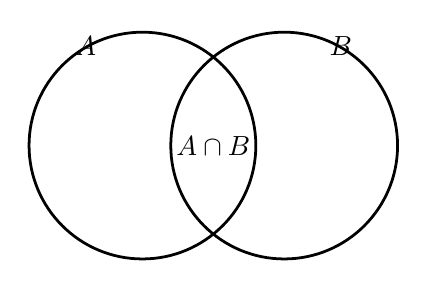
\begin{tikzpicture}[x=0.9cm,y=0.9cm,line width=1pt]
    \draw (-1,0) circle (1.6);
    \draw (1,0) circle (1.6);
    \node at (-1.8,1.4) {\(A\)};
    \node at (1.8,1.4) {\(B\)};
    \node at (0,0) {\(A\cap B\)};
\end{tikzpicture}}
\end{center}

\begin{exemple}
Dans un lycée, \(28\) élèves pratiquent le football, \(19\) pratiquent le
basket-ball et \(8\) pratiquent les deux sports.
\end{exemple}

\begin{solution}
Le nombre d'élèves pratiquant au moins l'un des deux sports est

\[
28+19-8=39.
\]

Ainsi,

\[
\boxed{39\text{ élèves pratiquent au moins un des deux sports}.}
\]

Sans le terme \(-8\), les \(8\) élèves pratiquant les deux sports seraient
comptés deux fois.
\end{solution}

\subsection{Compter par le complémentaire}\label{sec:complementaire}

\begin{proposition}[Passage au complémentaire]\label{prop:complementaire}
Soit \(E\) l'ensemble fini de toutes les possibilités, et soit \(A\) l'ensemble des
cas interdits (contenu dans \(E\)). On note \(E\setminus A\) l'ensemble des éléments de \(E\)
qui ne sont pas dans \(A\) : ce sont les cas valides.

Alors
\[
\boxed{
|E\setminus A|
=
|E|-|A|
}
\]
\end{proposition}

\begin{exemple}
On forme un code de \(4\) chiffres à l'aide des chiffres
\[
0,1,2,\dots,9.
\]
Il y a au total
\[
10^4
\]
codes.

Les codes ne contenant aucun \(7\) sont au nombre de
\[
9^4.
\]

Le nombre de codes contenant au moins un \(7\) est donc
\[
\boxed{10^4-9^4=3439.}
\]
\end{exemple}

\subsection{Retour aux trois fokontany}\label{sec:retour-trois-fokontany}

\begin{exemple}
Trois fokontany \(A\), \(B\) et \(C\) présentent chacun \(4\) candidats.
On veut former un comité de \(5\) personnes dans lequel chaque fokontany est
représenté.
\end{exemple}

\begin{solution}
Il y a au total
\[
\binom{12}{5}
\]
comités.

Notons, pour les comités de \(5\) personnes :
\begin{itemize}
    \item \(E_A\) : les comités ne contenant personne du fokontany \(A\) ;
    \item \(E_B\) : les comités ne contenant personne du fokontany \(B\) ;
    \item \(E_C\) : les comités ne contenant personne du fokontany \(C\).
\end{itemize}

Pour chacun de ces ensembles, on choisit les \(5\) membres parmi les \(8\)
candidats des deux autres fokontany :
\[
|E_A|=|E_B|=|E_C|=\binom{8}{5}.
\]

Il est impossible que deux fokontany soient simultanément absents, car il
faudrait choisir \(5\) personnes parmi les \(4\) candidats du fokontany restant.

Ainsi,
\[
|E_A\cap E_B|
=
|E_A\cap E_C|
=
|E_B\cap E_C|
=
0.
\]

Ces trois ensembles n'ont donc aucun comité en commun : par le principe additif, le nombre de
comités où au moins un fokontany est absent est \(|E_A|+|E_B|+|E_C|=3\binom{8}{5}\).
Le nombre de comités valides est donc
\[
\boxed{
\binom{12}{5}
-
3\binom{8}{5}
=
624.
}
\]
\end{solution}

\begin{remarque}
Il s'agit déjà d'une application du principe d'inclusion--exclusion.
\end{remarque}

\subsection{Trois ensembles}\label{sec:trois-ensembles}

\begin{theoreme}[Inclusion--exclusion pour trois ensembles]\label{thm:ie-trois}
Soient \(A\), \(B\) et \(C\) trois ensembles finis. Alors
\[
\boxed{
\begin{aligned}
|A\cup B\cup C|
={}&|A|+|B|+|C|\\
&-|A\cap B|-|A\cap C|-|B\cap C|\\
&+|A\cap B\cap C|.
\end{aligned}
}
\]
\end{theoreme}

\begin{proof}
Pour trois ensembles \(A\), \(B\) et \(C\), on commence par additionner leurs
tailles :
\[
|A|+|B|+|C|.
\]

Tout élément appartenant exactement à deux ensembles a été compté deux fois. Un élément appartenant aux trois ensembles a été compté trois fois.
On retranche donc une fois chaque intersection de deux ensembles :
\[
|A|+|B|+|C|-|A\cap B|-|A\cap C|-|B\cap C|.
\]

Un élément qui est dans exactement deux ensembles est maintenant compté une seule fois.
Mais les éléments de \(A\cap B\cap C\) ont alors été :
\begin{itemize}
    \item comptés trois fois au début ;
    \item puis retranchés trois fois.
\end{itemize}

Ils ne sont donc plus comptés du tout. Il faut les ajouter une fois, ce qui donne la formule.
\end{proof}

\begin{remarque}
Les signes alternent :
\[
\resizebox{\linewidth}{!}{$\displaystyle
\boxed{
+\text{ ensembles seuls}
\quad
-\text{ intersections de deux ensembles}
\quad
+\text{ intersection des trois ensembles}.
}
$}
\]

Avec plus de trois ensembles, on continue de la même façon : on ajoute les tailles des
ensembles, on retranche celles des intersections de deux ensembles, on ajoute celles des
intersections de trois ensembles, on retranche celles des intersections de quatre ensembles, etc.
\end{remarque}

\subsection{Forme complémentaire}\label{sec:forme-complementaire}

\begin{proposition}[Forme complémentaire]\label{prop:forme-complementaire}
Si \(E\) est l'ensemble fini de toutes les possibilités et si \(A\), \(B\), \(C\)
(contenus dans \(E\)) désignent trois catégories de cas interdits, alors le nombre de cas valides est
\(|E\setminus(A\cup B\cup C)|\), et, par inclusion--exclusion,
\[
\boxed{
\begin{aligned}
|E\setminus(A\cup B\cup C)|
={}&|E|-|A|-|B|-|C|\\
&+|A\cap B|+|A\cap C|+|B\cap C|\\
&-|A\cap B\cap C|.
\end{aligned}
}
\]
\end{proposition}

\subsection{Exemple numérique}\label{sec:exemple-numerique}

\begin{exemple}
Parmi les entiers de \(1\) à \(100\), combien sont divisibles par \(2\) ou par
\(5\) ?
\end{exemple}

\begin{solution}
Notons :
\[
A=\{\text{multiples de }2\},
\qquad
B=\{\text{multiples de }5\}.
\]

On a
\[
|A|=50,
\qquad
|B|=20.
\]

Les nombres divisibles à la fois par \(2\) et par \(5\) sont les multiples de
\(10\) :
\[
|A\cap B|=10.
\]

Ainsi,
\[
|A\cup B|
=
50+20-10
=
60.
\]

Donc
\[
\boxed{60\text{ entiers sont divisibles par }2\text{ ou par }5.}
\]

Le nombre d'entiers qui ne sont divisibles ni par \(2\), ni par \(5\), est
\[
100-60=40.
\]
\end{solution}

\begin{retenir}
\[
\boxed{
\text{On additionne les cas simples,}
}
\]

\[
\boxed{
\text{on retranche les doubles intersections,}
}
\]

\[
\boxed{
\text{on ajoute les triples intersections, etc.}
}
\]

Le principe général repose sur une alternance de signes :
\[
\boxed{
+\quad -\quad +\quad -\quad \cdots
}
\]
\end{retenir}

\subsection*{Exercices de compréhension}

% Note d'origine : « Exercice de compréhension »
\exochap{recueil-6-langues-classe}{Les langues d'une classe}

\subsection*{Exercices \texorpdfstring{$+$}{+}}

% Note d'origine : « Exercice + »
\exochap{recueil-6-divisibles-3-5}{Divisibles par 3 ou par 5}

\subsection*{Exercices \texorpdfstring{$++$}{++}}

% Note d'origine : « Exercice ++ »
\exercice{recueil-6-quatre-fokontany}{Quatre fokontany}

% ------------------------------------------------------------
\section{Concept : les bijections}\label{sec:bijections}

Une méthode fondamentale en combinatoire consiste à remplacer les objets
que l'on souhaite compter par d'autres objets, plus simples à dénombrer.

\subsection{Exemple introductif : Soa, Tovo, Fara, Hery et les mots binaires}\label{sec:exemple-mots-binaires}

On considère l'ensemble de quatre élèves
\[
E=\{\text{Soa},\text{Tovo},\text{Fara},\text{Hery}\}.
\]

On souhaite former un comité en choisissant certains de ces élèves.
Le comité peut éventuellement être vide.

On fixe l'ordre suivant :
\[
(\text{Soa},\text{Tovo},\text{Fara},\text{Hery}).
\]

À chaque comité, on associe un mot de quatre chiffres composé de \(0\) et de
\(1\) :

\begin{itemize}
    \item on écrit \(1\) lorsque l'élève appartient au comité ;
    \item on écrit \(0\) lorsque l'élève n'appartient pas au comité.
\end{itemize}

Par exemple,
\[
\{\text{Soa},\text{Fara}\}
\longleftrightarrow
1010.
\]

\begin{center}
\fitfig{%
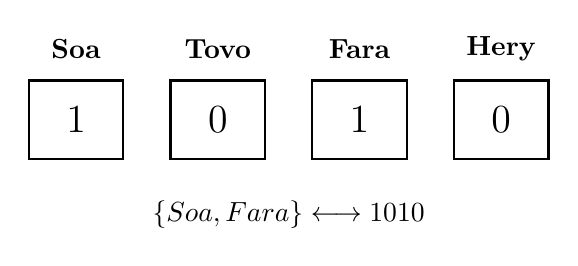
\begin{tikzpicture}[x=1cm,y=1cm,line width=0.8pt]
    \node at (0.75,1.8){\textbf{Soa}};
    \node at (2.55,1.8){\textbf{Tovo}};
    \node at (4.35,1.8){\textbf{Fara}};
    \node at (6.15,1.8){\textbf{Hery}};
    \draw (0.15,0.4) rectangle (1.35,1.4);
    \draw (1.95,0.4) rectangle (3.15,1.4);
    \draw (3.75,0.4) rectangle (4.95,1.4);
    \draw (5.55,0.4) rectangle (6.75,1.4);
    \node at (0.75,0.9){\Large \(1\)};
    \node at (2.55,0.9){\Large \(0\)};
    \node at (4.35,0.9){\Large \(1\)};
    \node at (6.15,0.9){\Large \(0\)};
    \node at (3.45,-0.3){\(\{\text{Soa},\text{Fara}\}\longleftrightarrow 1010\)};
\end{tikzpicture}}
\end{center}

De même,
\[
\{\text{Tovo},\text{Fara},\text{Hery}\}
\longleftrightarrow
0111,
\]

\[
\varnothing
\longleftrightarrow
0000,
\]

et
\[
E
\longleftrightarrow
1111.
\]

Chaque comité donne un unique mot binaire, et chaque mot binaire détermine
un unique comité.

Comme chacune des quatre positions possède deux possibilités, \(0\) ou \(1\),
le nombre de mots binaires est
\[
2\times2\times2\times2=2^4=16.
\]

Il existe donc également \(16\) comités possibles.

Plus généralement, pour un ensemble de \(n\) personnes, chaque sous-ensemble
correspond à un mot binaire de longueur \(n\). Par conséquent,

\begin{proposition}[Nombre de sous-ensembles]\label{prop:sous-ensembles}
Un ensemble à \(n\) éléments possède \(2^n\) sous-ensembles.
\end{proposition}

\subsection{Le concept : une correspondance un-à-un pour compter}\label{sec:concept-bijection}

\begin{definition}[Bijection]\label{def:bijection}
Une \emph{bijection} entre deux ensembles \(\mathcal A\) et \(\mathcal B\)
est une correspondance telle que :

\begin{itemize}
    \item chaque élément de \(\mathcal A\) correspond à un unique élément de
    \(\mathcal B\) ;
    \item chaque élément de \(\mathcal B\) correspond à un unique élément de
    \(\mathcal A\).
\end{itemize}
\end{definition}

Il s'agit donc d'une correspondance parfaite, \emph{un objet contre un objet}.

\begin{center}
\fitfig{%
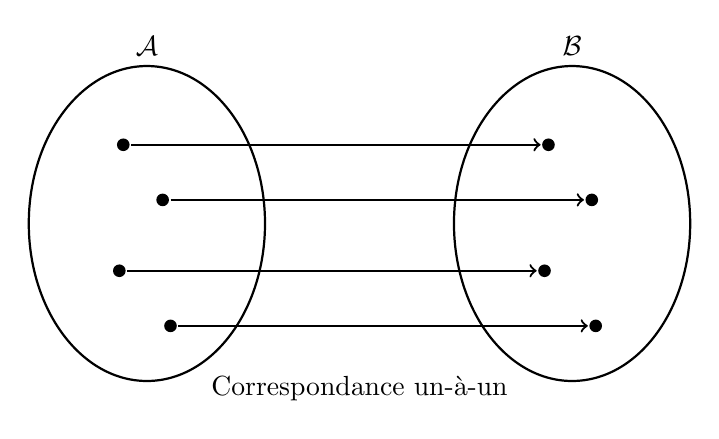
\begin{tikzpicture}[x=1cm,y=1cm,line width=0.8pt]
    \draw (1.7,2) ellipse (1.5 and 2);
    \draw (7.1,2) ellipse (1.5 and 2);
    \node at (1.7,4.25){\(\mathcal A\)};
    \node at (7.1,4.25){\(\mathcal B\)};
    \fill (1.4,3) circle (0.08);
    \fill (1.9,2.3) circle (0.08);
    \fill (1.35,1.4) circle (0.08);
    \fill (2,0.7) circle (0.08);
    \fill (6.8,3) circle (0.08);
    \fill (7.35,2.3) circle (0.08);
    \fill (6.75,1.4) circle (0.08);
    \fill (7.4,0.7) circle (0.08);
    \draw[->] (1.5,3)--(6.7,3);
    \draw[->] (2,2.3)--(7.25,2.3);
    \draw[->] (1.45,1.4)--(6.65,1.4);
    \draw[->] (2.1,0.7)--(7.3,0.7);
    \node at (4.4,-0.1){Correspondance un-à-un};
\end{tikzpicture}}
\end{center}

\begin{proposition}[Bijection et nombre d'éléments]\label{prop:bijection-cardinal}
Lorsqu'il existe une bijection entre deux ensembles finis, ces deux ensembles
ont le même nombre d'éléments :
\[
\boxed{
\mathcal A\longleftrightarrow\mathcal B
\qquad\Longrightarrow\qquad
|\mathcal A|=|\mathcal B|.
}
\]
\end{proposition}

\begin{methode}[Stratégie de comptage]
La stratégie de comptage est la suivante : pour compter une famille d'objets compliqués,
on construit une bijection avec une famille d'objets plus faciles à compter.
\[
\boxed{
\text{objets compliqués}
\longleftrightarrow
\text{objets simples}
}
\]
\end{methode}

Dans l'exemple précédent,
\[
\boxed{
\text{comités formés parmi \(n\) personnes}
\longleftrightarrow
\text{mots binaires de longueur \(n\)}.
}
\]

\begin{retenir}
Une bijection permet de compter une famille d'objets en la mettant en
correspondance parfaite avec une autre famille dont le nombre d'éléments est
déjà connu ou plus facile à déterminer.

\[
\boxed{
\mathcal A\longleftrightarrow\mathcal B
\quad\Longrightarrow\quad
|\mathcal A|=|\mathcal B|
}
\]
\end{retenir}

\subsection*{Exercices}

% Note d'origine : « Un premier exercice simple »
\exercice{recueil-6-comites-mots-binaires}{Comités et mots binaires}

% Note d'origine : « Chemins sur un quadrillage et coefficient binomial $\binom{p+q}{p}$ »
\exercice{recueil-6-chemins-quadrillage}{Chemins sur un quadrillage}

% Note d'origine : « Partitionner $2n$ personnes en $n$ binômes »
\exercice{recueil-6-binomes}{Partitionner \texorpdfstring{$2n$}{2n} personnes en \texorpdfstring{$n$}{n} binômes}

% ------------------------------------------------------------
\section{À retenir}\label{sec:retenir}

\begin{retenir}
\begin{itemize}
    \item \textbf{Additif et multiplicatif :} on additionne quand le choix se fait \emph{ceci ou cela}
    (sans choix commun), on multiplie quand il se fait \emph{ceci puis cela} ; un arbre des choix
    aide à visualiser le comptage.
    \item \textbf{Codes :} \(n^p\) avec répétition, \(n(n-1)\cdots(n-p+1)\) sans répétition (\(p\le n\)).
    \item \textbf{Rangements :} \(n!\) permutations de \(n\) objets distincts ;
    \(\dfrac{n!}{(n-k)!}\) choix ordonnés de \(k\) objets parmi \(n\) ;
    \(\dbinom{n}{k}=\dfrac{n!}{k!\,(n-k)!}\) choix sans ordre.
    \item \textbf{Anagrammes :} avec des objets identiques, \(\dfrac{n!}{n_1!\,n_2!\cdots n_r!}\) rangements.
    \item \textbf{Inclusion--exclusion :}
    \(|A\cup B|=|A|+|B|-|A\cap B|\) ; pour trois ensembles, les signes alternent
    \(+\,-\,+\) ; on compte aussi par le complémentaire : \(|E\setminus A|=|E|-|A|\).
    \item \textbf{Bijections :} deux ensembles finis en bijection ont le même nombre d'éléments ;
    on remplace des objets compliqués par des objets plus simples à compter
    (comités \(\leftrightarrow\) mots binaires : \(2^n\) sous-ensembles d'un ensemble à \(n\) éléments).
\end{itemize}
\end{retenir}

% Aucune solution rédigée à ce jour (a_solution: false pour les 8 exercices) :
% la section « Solutions » (\solutionde{id}{titre}{ex|exo}) sera ajoutée avec les solution.tex.

\end{document}
